% Options for packages loaded elsewhere
\PassOptionsToPackage{unicode}{hyperref}
\PassOptionsToPackage{hyphens}{url}
%
\documentclass[
]{article}
\title{NWFSC HL Survey Index for Vermilion in 2021}
\author{}
\date{\vspace{-2.5em}July 10, 2021}

\usepackage{amsmath,amssymb}
\usepackage{lmodern}
\usepackage{iftex}
\ifPDFTeX
  \usepackage[T1]{fontenc}
  \usepackage[utf8]{inputenc}
  \usepackage{textcomp} % provide euro and other symbols
\else % if luatex or xetex
  \usepackage{unicode-math}
  \defaultfontfeatures{Scale=MatchLowercase}
  \defaultfontfeatures[\rmfamily]{Ligatures=TeX,Scale=1}
\fi
% Use upquote if available, for straight quotes in verbatim environments
\IfFileExists{upquote.sty}{\usepackage{upquote}}{}
\IfFileExists{microtype.sty}{% use microtype if available
  \usepackage[]{microtype}
  \UseMicrotypeSet[protrusion]{basicmath} % disable protrusion for tt fonts
}{}
\makeatletter
\@ifundefined{KOMAClassName}{% if non-KOMA class
  \IfFileExists{parskip.sty}{%
    \usepackage{parskip}
  }{% else
    \setlength{\parindent}{0pt}
    \setlength{\parskip}{6pt plus 2pt minus 1pt}}
}{% if KOMA class
  \KOMAoptions{parskip=half}}
\makeatother
\usepackage{xcolor}
\IfFileExists{xurl.sty}{\usepackage{xurl}}{} % add URL line breaks if available
\IfFileExists{bookmark.sty}{\usepackage{bookmark}}{\usepackage{hyperref}}
\hypersetup{
  pdftitle={NWFSC HL Survey Index for Vermilion in 2021},
  hidelinks,
  pdfcreator={LaTeX via pandoc}}
\urlstyle{same} % disable monospaced font for URLs
\usepackage[margin=1in]{geometry}
\usepackage{longtable,booktabs,array}
\usepackage{calc} % for calculating minipage widths
% Correct order of tables after \paragraph or \subparagraph
\usepackage{etoolbox}
\makeatletter
\patchcmd\longtable{\par}{\if@noskipsec\mbox{}\fi\par}{}{}
\makeatother
% Allow footnotes in longtable head/foot
\IfFileExists{footnotehyper.sty}{\usepackage{footnotehyper}}{\usepackage{footnote}}
\makesavenoteenv{longtable}
\usepackage{graphicx}
\makeatletter
\def\maxwidth{\ifdim\Gin@nat@width>\linewidth\linewidth\else\Gin@nat@width\fi}
\def\maxheight{\ifdim\Gin@nat@height>\textheight\textheight\else\Gin@nat@height\fi}
\makeatother
% Scale images if necessary, so that they will not overflow the page
% margins by default, and it is still possible to overwrite the defaults
% using explicit options in \includegraphics[width, height, ...]{}
\setkeys{Gin}{width=\maxwidth,height=\maxheight,keepaspectratio}
% Set default figure placement to htbp
\makeatletter
\def\fps@figure{htbp}
\makeatother
\setlength{\emergencystretch}{3em} % prevent overfull lines
\providecommand{\tightlist}{%
  \setlength{\itemsep}{0pt}\setlength{\parskip}{0pt}}
\setcounter{secnumdepth}{5}
\usepackage{booktabs}
\usepackage{longtable}
\usepackage{array}
\usepackage{multirow}
\usepackage{wrapfig}
\usepackage{float}
\usepackage{colortbl}
\usepackage{pdflscape}
\usepackage{tabu}
\usepackage{threeparttable}
\usepackage[normalem]{ulem}
\usepackage{makecell}
\usepackage{xcolor}
\usepackage{placeins}
\ifLuaTeX
  \usepackage{selnolig}  % disable illegal ligatures
\fi

\begin{document}
\maketitle

{
\setcounter{tocdepth}{2}
\tableofcontents
}
\hypertarget{northwest-fisheries-science-center-hook-and-line-survey}{%
\subsubsection{Northwest Fisheries Science Center Hook-and-Line Survey}\label{northwest-fisheries-science-center-hook-and-line-survey}}

Since 2004, the NWFSC has conducted an annual hook-and-line survey targeting shelf rockfish at fixed stations (`sites') in the Southern California Bight (Figure \ref{fig:spp-sites}). During each site visit, three deckhands simultaneously deploy 5-hook sampling rigs (this is referred to as a single `drop') for a maximum of 5 minutes per line, but individual lines may be retrieved sooner at the angler's discretion (e.g.~to avoid losing fish). Five drops are attempted at each site for a maximum possible catch of 75 fish per site per year (3 anglers × 5 hooks × 5 drops). Further details regarding the sampling frame, site selection, and survey methodology are described by {[}-@Harms2008{]}.

From 2004 through 2013, sampling was conducted only outside the Cowcod Conservation Areas. Beginning in 2014, 40 sites inside the CCAs were sampled, and roughly another 40 sites have been added in subsequent years inside the CCAs. The survey currently has 201 sites (79 inside and 122 outside the CCAs).

\textbf{Northwest Fisheries Science Center Hook-and-Line Survey Index: Data Preparation, Filtering, and Sample Sizes}

Vermilion is one of the most commonly encountered species in the NWFSC hook-and-line survey {[}Harms 2008{]} (Figure \ref{fig:spp-sites}). Sites considered for an abundance index were limited to those that have caught at least 1 vermilion rockfish over the period 2004-2018 (circles in Figure xx ). Only 14 sites were identified as catching no vermilion over the entire sampling period. Sample sizes by depth and year can be found in Tables
\ref{tab:tab-depth-nwfschl} and \ref{tab:tab-year-nwfschl}.
Note that depth was used as a continuous variable (second-order polynomial) in the model, and depth bins were created for descriptive purposes and data exploration only.

\emph{Northwest Fisheries Science Center Hook-and-Line Survey Index: Model Selection, Fits, and Diagnostics}

The STAT explored alternative model structures to generate a standardized index of relative abundance. This included alternative response variables (catch in weight, catch in numbers, presence/absence), levels of aggregation (hook, drop, or site), probability distributions (binomial, negative binomial, lognormal, delta-gamma, and logit-normal), and covariates (year, site number, depth, distance to port, area, inside/outside CCA). Preliminary analyses showed that trends in the annual proportion of positive hooks were very similar to trends in catch rate per drop or site. Posterior predictive checks of annual means and standard deviations identified the logit-normal model as the most appropriate error distribution. The final model included covariate terms for year, site number, drop number, a
Second-order depth term, and a normally-distributed random effect for each observation.

Models were fit using the ``rstanarm'' R package (version 2.21.1). Posterior predictive
checks of the Bayesian model fit for the final logit model
were all reasonable (Figures \ref{fig:fig-posterior-mean-nwfschl} and
\ref{fig:fig-posterior-sd-nwfschl}). The model generated data sets with the
proportion zeros similar to the \textasciitilde50\% zeroes in the data
(Figure \ref{fig:fig-propzero-nwfschl}). The predicted marginal effects from
the final logit normal model can be found in Figure \ref{fig:marginal-nwfschl}.
The marginal depth effect represents the influence of depth on the proportion of vermilion \emph{after} accounting for site effects. A model
run without the site effect confirms that that depth follows the expected pattern
observed in the data, i.e.~a peak near 145 m (Figure \ref{fig:marginal2-nwfschl}).
The final index (Table \ref{tab:tab-index-nwfschl}),
when compared to the arithmetic mean of the annual CPUE, declines slightly more from 2008-2012, with a significant increase after 2016 (Figure \ref{fig:fig-cpue-nwfschl}).

The expansion of the survey area into the CCAs after 2014 limits exploration of year/area interactions in the model. The STAT adopted an approach similar to that used for the 2019 assessment of cowcod {[}@Dick2019{]}. Specifically, because site effects (both inside and outside the CCA) are constant over time in the index, selectivity for the index is estimated using composition data that represents all areas (2014-2019, inside and outside the CCAs). Not wanting to lose length and age compositions prior to 2014, these data are moved to a `dummy' fleet in the assessment model, and allowed to have a different selectivity curve due to differences in size composition inside and outside the CCAs {[}@Keller2019{]}. This treatment of the data, although not ideal, was seen as preferable to development of two separate indices.

\newpage

\begin{table}

\caption{\label{tab:tab-depth-nwfschl}Positive samples of vermilion in the southern model by depth (fm).}
\centering
\begin{tabular}[t]{lrrl}
\toprule
Year & Positive Samples & Samples & Percent Positive\\
\midrule
\cellcolor{gray!6}{(0,50]} & \cellcolor{gray!6}{85} & \cellcolor{gray!6}{295} & \cellcolor{gray!6}{29\%}\\
(50,75] & 226 & 815 & 28\%\\
\cellcolor{gray!6}{(75,100]} & \cellcolor{gray!6}{1697} & \cellcolor{gray!6}{3847} & \cellcolor{gray!6}{44\%}\\
(100,125] & 1278 & 2156 & 59\%\\
\cellcolor{gray!6}{(125,150]} & \cellcolor{gray!6}{917} & \cellcolor{gray!6}{1594} & \cellcolor{gray!6}{58\%}\\
\addlinespace
(150,175] & 663 & 1155 & 57\%\\
\cellcolor{gray!6}{(175,200]} & \cellcolor{gray!6}{234} & \cellcolor{gray!6}{456} & \cellcolor{gray!6}{51\%}\\
(200,235] & 75 & 122 & 61\%\\
\bottomrule
\end{tabular}
\end{table}

\begin{table}

\caption{\label{tab:tab-depthsite-nwfschl}Samples of vermilion in the
                                  NWFSC hook-and-line survey by area and 
                                  depth bins (ft).}
\centering
\resizebox{\linewidth}{!}{
\begin{tabular}[t]{lllllllll}
\toprule
Area name & (0,50] & (50,75] & (75,100] & (100,125] & (125,150] & (150,175] & (175,200] & (200,235]\\
\midrule
\cellcolor{gray!6}{Fourteen Mile Bank} & \cellcolor{gray!6}{} & \cellcolor{gray!6}{} & \cellcolor{gray!6}{0\%} & \cellcolor{gray!6}{7\%} & \cellcolor{gray!6}{38\%} & \cellcolor{gray!6}{32\%} & \cellcolor{gray!6}{21\%} & \cellcolor{gray!6}{}\\
107 and 118 Banks &  &  &  &  &  &  & 26\% & 10\%\\
\cellcolor{gray!6}{109 Bank} & \cellcolor{gray!6}{} & \cellcolor{gray!6}{} & \cellcolor{gray!6}{} & \cellcolor{gray!6}{} & \cellcolor{gray!6}{} & \cellcolor{gray!6}{50\%} & \cellcolor{gray!6}{71\%} & \cellcolor{gray!6}{50\%}\\
43 Fathom Bank &  &  & 22\% & 87\% &  &  & 4\% & 50\%\\
\cellcolor{gray!6}{Anacapa Island} & \cellcolor{gray!6}{} & \cellcolor{gray!6}{0\%} & \cellcolor{gray!6}{34\%} & \cellcolor{gray!6}{18\%} & \cellcolor{gray!6}{30\%} & \cellcolor{gray!6}{9\%} & \cellcolor{gray!6}{0\%} & \cellcolor{gray!6}{}\\
\addlinespace
Catalina Island &  & 13\% & 45\% &  & 67\% & 55\% & 21\% & \\
\cellcolor{gray!6}{Central Coast} & \cellcolor{gray!6}{} & \cellcolor{gray!6}{} & \cellcolor{gray!6}{34\%} & \cellcolor{gray!6}{40\%} & \cellcolor{gray!6}{8\%} & \cellcolor{gray!6}{14\%} & \cellcolor{gray!6}{} & \cellcolor{gray!6}{}\\
Cherry Bank &  &  & 82\% & 77\% & 59\% & 72\% & 55\% & \\
\cellcolor{gray!6}{Cortez Bank} & \cellcolor{gray!6}{} & \cellcolor{gray!6}{11\%} & \cellcolor{gray!6}{50\%} & \cellcolor{gray!6}{94\%} & \cellcolor{gray!6}{79\%} & \cellcolor{gray!6}{62\%} & \cellcolor{gray!6}{100\%} & \cellcolor{gray!6}{100\%}\\
Garrett Bank &  &  &  & 100\% & 100\% & 58\% & 78\% & 89\%\\
\addlinespace
\cellcolor{gray!6}{Harrison Reef} & \cellcolor{gray!6}{} & \cellcolor{gray!6}{} & \cellcolor{gray!6}{11\%} & \cellcolor{gray!6}{53\%} & \cellcolor{gray!6}{50\%} & \cellcolor{gray!6}{} & \cellcolor{gray!6}{} & \cellcolor{gray!6}{}\\
Hidden Reef &  &  &  & 35\% & 80\% &  &  & \\
\cellcolor{gray!6}{Kidney Bank} & \cellcolor{gray!6}{} & \cellcolor{gray!6}{} & \cellcolor{gray!6}{} & \cellcolor{gray!6}{82\%} & \cellcolor{gray!6}{37\%} & \cellcolor{gray!6}{58\%} & \cellcolor{gray!6}{} & \cellcolor{gray!6}{}\\
Nine Mile Bank &  &  &  & 38\% & 70\% & 25\% &  & \\
\cellcolor{gray!6}{Osborn Bank} & \cellcolor{gray!6}{0\%} & \cellcolor{gray!6}{20\%} & \cellcolor{gray!6}{10\%} & \cellcolor{gray!6}{} & \cellcolor{gray!6}{} & \cellcolor{gray!6}{88\%} & \cellcolor{gray!6}{} & \cellcolor{gray!6}{}\\
\addlinespace
Point Conception/Arguello &  &  & 93\% & 90\% & 85\% & 100\% & 100\% & \\
\cellcolor{gray!6}{Port Hueneme} & \cellcolor{gray!6}{} & \cellcolor{gray!6}{} & \cellcolor{gray!6}{66\%} & \cellcolor{gray!6}{} & \cellcolor{gray!6}{} & \cellcolor{gray!6}{} & \cellcolor{gray!6}{} & \cellcolor{gray!6}{}\\
Potato Bank &  &  & 80\% & 46\% & 16\% & 80\% & 80\% & \\
\cellcolor{gray!6}{San Clemente Island} & \cellcolor{gray!6}{10\%} & \cellcolor{gray!6}{0\%} & \cellcolor{gray!6}{27\%} & \cellcolor{gray!6}{52\%} & \cellcolor{gray!6}{42\%} & \cellcolor{gray!6}{51\%} & \cellcolor{gray!6}{100\%} & \cellcolor{gray!6}{}\\
San Miguel Island &  & 50\% & 77\% & 98\% & 100\% &  &  & \\
\addlinespace
\cellcolor{gray!6}{San Nicolas Island East} & \cellcolor{gray!6}{} & \cellcolor{gray!6}{50\%} & \cellcolor{gray!6}{56\%} & \cellcolor{gray!6}{33\%} & \cellcolor{gray!6}{} & \cellcolor{gray!6}{75\%} & \cellcolor{gray!6}{} & \cellcolor{gray!6}{}\\
San Nicolas Island West &  & 57\% & 61\% & 78\% & 90\% & 74\% & 82\% & \\
\cellcolor{gray!6}{San Pedro Bay} & \cellcolor{gray!6}{} & \cellcolor{gray!6}{35\%} & \cellcolor{gray!6}{31\%} & \cellcolor{gray!6}{} & \cellcolor{gray!6}{} & \cellcolor{gray!6}{} & \cellcolor{gray!6}{} & \cellcolor{gray!6}{}\\
Santa Barbara & 24\% & 65\% & 66\% &  &  &  &  & \\
\cellcolor{gray!6}{Santa Barbara Channel} & \cellcolor{gray!6}{} & \cellcolor{gray!6}{} & \cellcolor{gray!6}{33\%} & \cellcolor{gray!6}{43\%} & \cellcolor{gray!6}{100\%} & \cellcolor{gray!6}{54\%} & \cellcolor{gray!6}{29\%} & \cellcolor{gray!6}{}\\
\addlinespace
Santa Barbara Island &  &  & 42\% & 85\% & 92\% & 65\% & 88\% & 67\%\\
\cellcolor{gray!6}{Santa Cruz Island} & \cellcolor{gray!6}{} & \cellcolor{gray!6}{10\%} & \cellcolor{gray!6}{32\%} & \cellcolor{gray!6}{} & \cellcolor{gray!6}{100\%} & \cellcolor{gray!6}{83\%} & \cellcolor{gray!6}{90\%} & \cellcolor{gray!6}{96\%}\\
Santa Monica Bay & 31\% & 17\% & 35\% & 14\% & 68\% &  &  & \\
\cellcolor{gray!6}{Santa Rosa Flats} & \cellcolor{gray!6}{} & \cellcolor{gray!6}{} & \cellcolor{gray!6}{} & \cellcolor{gray!6}{66\%} & \cellcolor{gray!6}{31\%} & \cellcolor{gray!6}{82\%} & \cellcolor{gray!6}{79\%} & \cellcolor{gray!6}{23\%}\\
Santa Rosa Island &  & 12\% & 64\% & 100\% &  &  &  & \\
\addlinespace
\cellcolor{gray!6}{Sixty Mile Bank} & \cellcolor{gray!6}{} & \cellcolor{gray!6}{} & \cellcolor{gray!6}{30\%} & \cellcolor{gray!6}{38\%} & \cellcolor{gray!6}{61\%} & \cellcolor{gray!6}{40\%} & \cellcolor{gray!6}{20\%} & \cellcolor{gray!6}{0\%}\\
South Coast & 52\% & 12\% & 29\% & 23\% & 0\% &  &  & \\
\cellcolor{gray!6}{Tanner Bank} & \cellcolor{gray!6}{} & \cellcolor{gray!6}{} & \cellcolor{gray!6}{53\%} & \cellcolor{gray!6}{62\%} & \cellcolor{gray!6}{100\%} & \cellcolor{gray!6}{100\%} & \cellcolor{gray!6}{93\%} & \cellcolor{gray!6}{100\%}\\
\bottomrule
\end{tabular}}
\end{table}

\begin{table}

\caption{\label{tab:tab-year-nwfschl}Samples of vermilion in the southern model by year.}
\centering
\begin{tabular}[t]{lrrl}
\toprule
Year & Positive Samples & Samples & Percent Positive\\
\midrule
\cellcolor{gray!6}{2004} & \cellcolor{gray!6}{184} & \cellcolor{gray!6}{363} & \cellcolor{gray!6}{51\%}\\
2005 & 210 & 442 & 48\%\\
\cellcolor{gray!6}{2006} & \cellcolor{gray!6}{187} & \cellcolor{gray!6}{448} & \cellcolor{gray!6}{42\%}\\
2007 & 205 & 490 & 42\%\\
\cellcolor{gray!6}{2008} & \cellcolor{gray!6}{227} & \cellcolor{gray!6}{577} & \cellcolor{gray!6}{39\%}\\
\addlinespace
2009 & 243 & 575 & 42\%\\
\cellcolor{gray!6}{2010} & \cellcolor{gray!6}{225} & \cellcolor{gray!6}{584} & \cellcolor{gray!6}{39\%}\\
2011 & 245 & 531 & 46\%\\
\cellcolor{gray!6}{2012} & \cellcolor{gray!6}{275} & \cellcolor{gray!6}{584} & \cellcolor{gray!6}{47\%}\\
2013 & 296 & 579 & 51\%\\
\addlinespace
\cellcolor{gray!6}{2014} & \cellcolor{gray!6}{381} & \cellcolor{gray!6}{744} & \cellcolor{gray!6}{51\%}\\
2015 & 470 & 880 & 53\%\\
\cellcolor{gray!6}{2016} & \cellcolor{gray!6}{438} & \cellcolor{gray!6}{858} & \cellcolor{gray!6}{51\%}\\
2017 & 537 & 916 & 59\%\\
\cellcolor{gray!6}{2018} & \cellcolor{gray!6}{543} & \cellcolor{gray!6}{934} & \cellcolor{gray!6}{58\%}\\
\addlinespace
2019 & 509 & 935 & 54\%\\
\bottomrule
\end{tabular}
\end{table}

\FloatBarrier

\begin{table}

\caption{\label{tab:tab-index-nwfschl}Standardized index for the NWFSC HL survey index with log-scale standard errors and 95% highest
       posterior density (HPD) intervals for vermilion in the southern model .}
\centering
\begin{tabular}[t]{rrrrr}
\toprule
Year & Mean & logSE & lower HPD & upper HPD\\
\midrule
\cellcolor{gray!6}{2004} & \cellcolor{gray!6}{0.0403} & \cellcolor{gray!6}{0.2824} & \cellcolor{gray!6}{0.0222} & \cellcolor{gray!6}{0.0666}\\
2005 & 0.0491 & 0.2768 & 0.0272 & 0.0798\\
\cellcolor{gray!6}{2006} & \cellcolor{gray!6}{0.0438} & \cellcolor{gray!6}{0.2817} & \cellcolor{gray!6}{0.0239} & \cellcolor{gray!6}{0.0719}\\
2007 & 0.0445 & 0.2790 & 0.0244 & 0.0722\\
\cellcolor{gray!6}{2008} & \cellcolor{gray!6}{0.0266} & \cellcolor{gray!6}{0.2843} & \cellcolor{gray!6}{0.0145} & \cellcolor{gray!6}{0.0444}\\
\addlinespace
2009 & 0.0355 & 0.2819 & 0.0195 & 0.0583\\
\cellcolor{gray!6}{2010} & \cellcolor{gray!6}{0.0361} & \cellcolor{gray!6}{0.2825} & \cellcolor{gray!6}{0.0197} & \cellcolor{gray!6}{0.0599}\\
2011 & 0.0532 & 0.2741 & 0.0295 & 0.0864\\
\cellcolor{gray!6}{2012} & \cellcolor{gray!6}{0.0454} & \cellcolor{gray!6}{0.2756} & \cellcolor{gray!6}{0.0254} & \cellcolor{gray!6}{0.0739}\\
2013 & 0.0526 & 0.2765 & 0.0290 & 0.0858\\
\addlinespace
\cellcolor{gray!6}{2014} & \cellcolor{gray!6}{0.0578} & \cellcolor{gray!6}{0.2697} & \cellcolor{gray!6}{0.0326} & \cellcolor{gray!6}{0.0931}\\
2015 & 0.0599 & 0.2661 & 0.0339 & 0.0957\\
\cellcolor{gray!6}{2016} & \cellcolor{gray!6}{0.0586} & \cellcolor{gray!6}{0.2697} & \cellcolor{gray!6}{0.0329} & \cellcolor{gray!6}{0.0950}\\
2017 & 0.0963 & 0.2562 & 0.0559 & 0.1511\\
\cellcolor{gray!6}{2018} & \cellcolor{gray!6}{0.0879} & \cellcolor{gray!6}{0.2606} & \cellcolor{gray!6}{0.0501} & \cellcolor{gray!6}{0.1392}\\
\addlinespace
2019 & 0.0674 & 0.2681 & 0.0381 & 0.1085\\
\bottomrule
\end{tabular}
\end{table}

\FloatBarrier

\begin{figure}
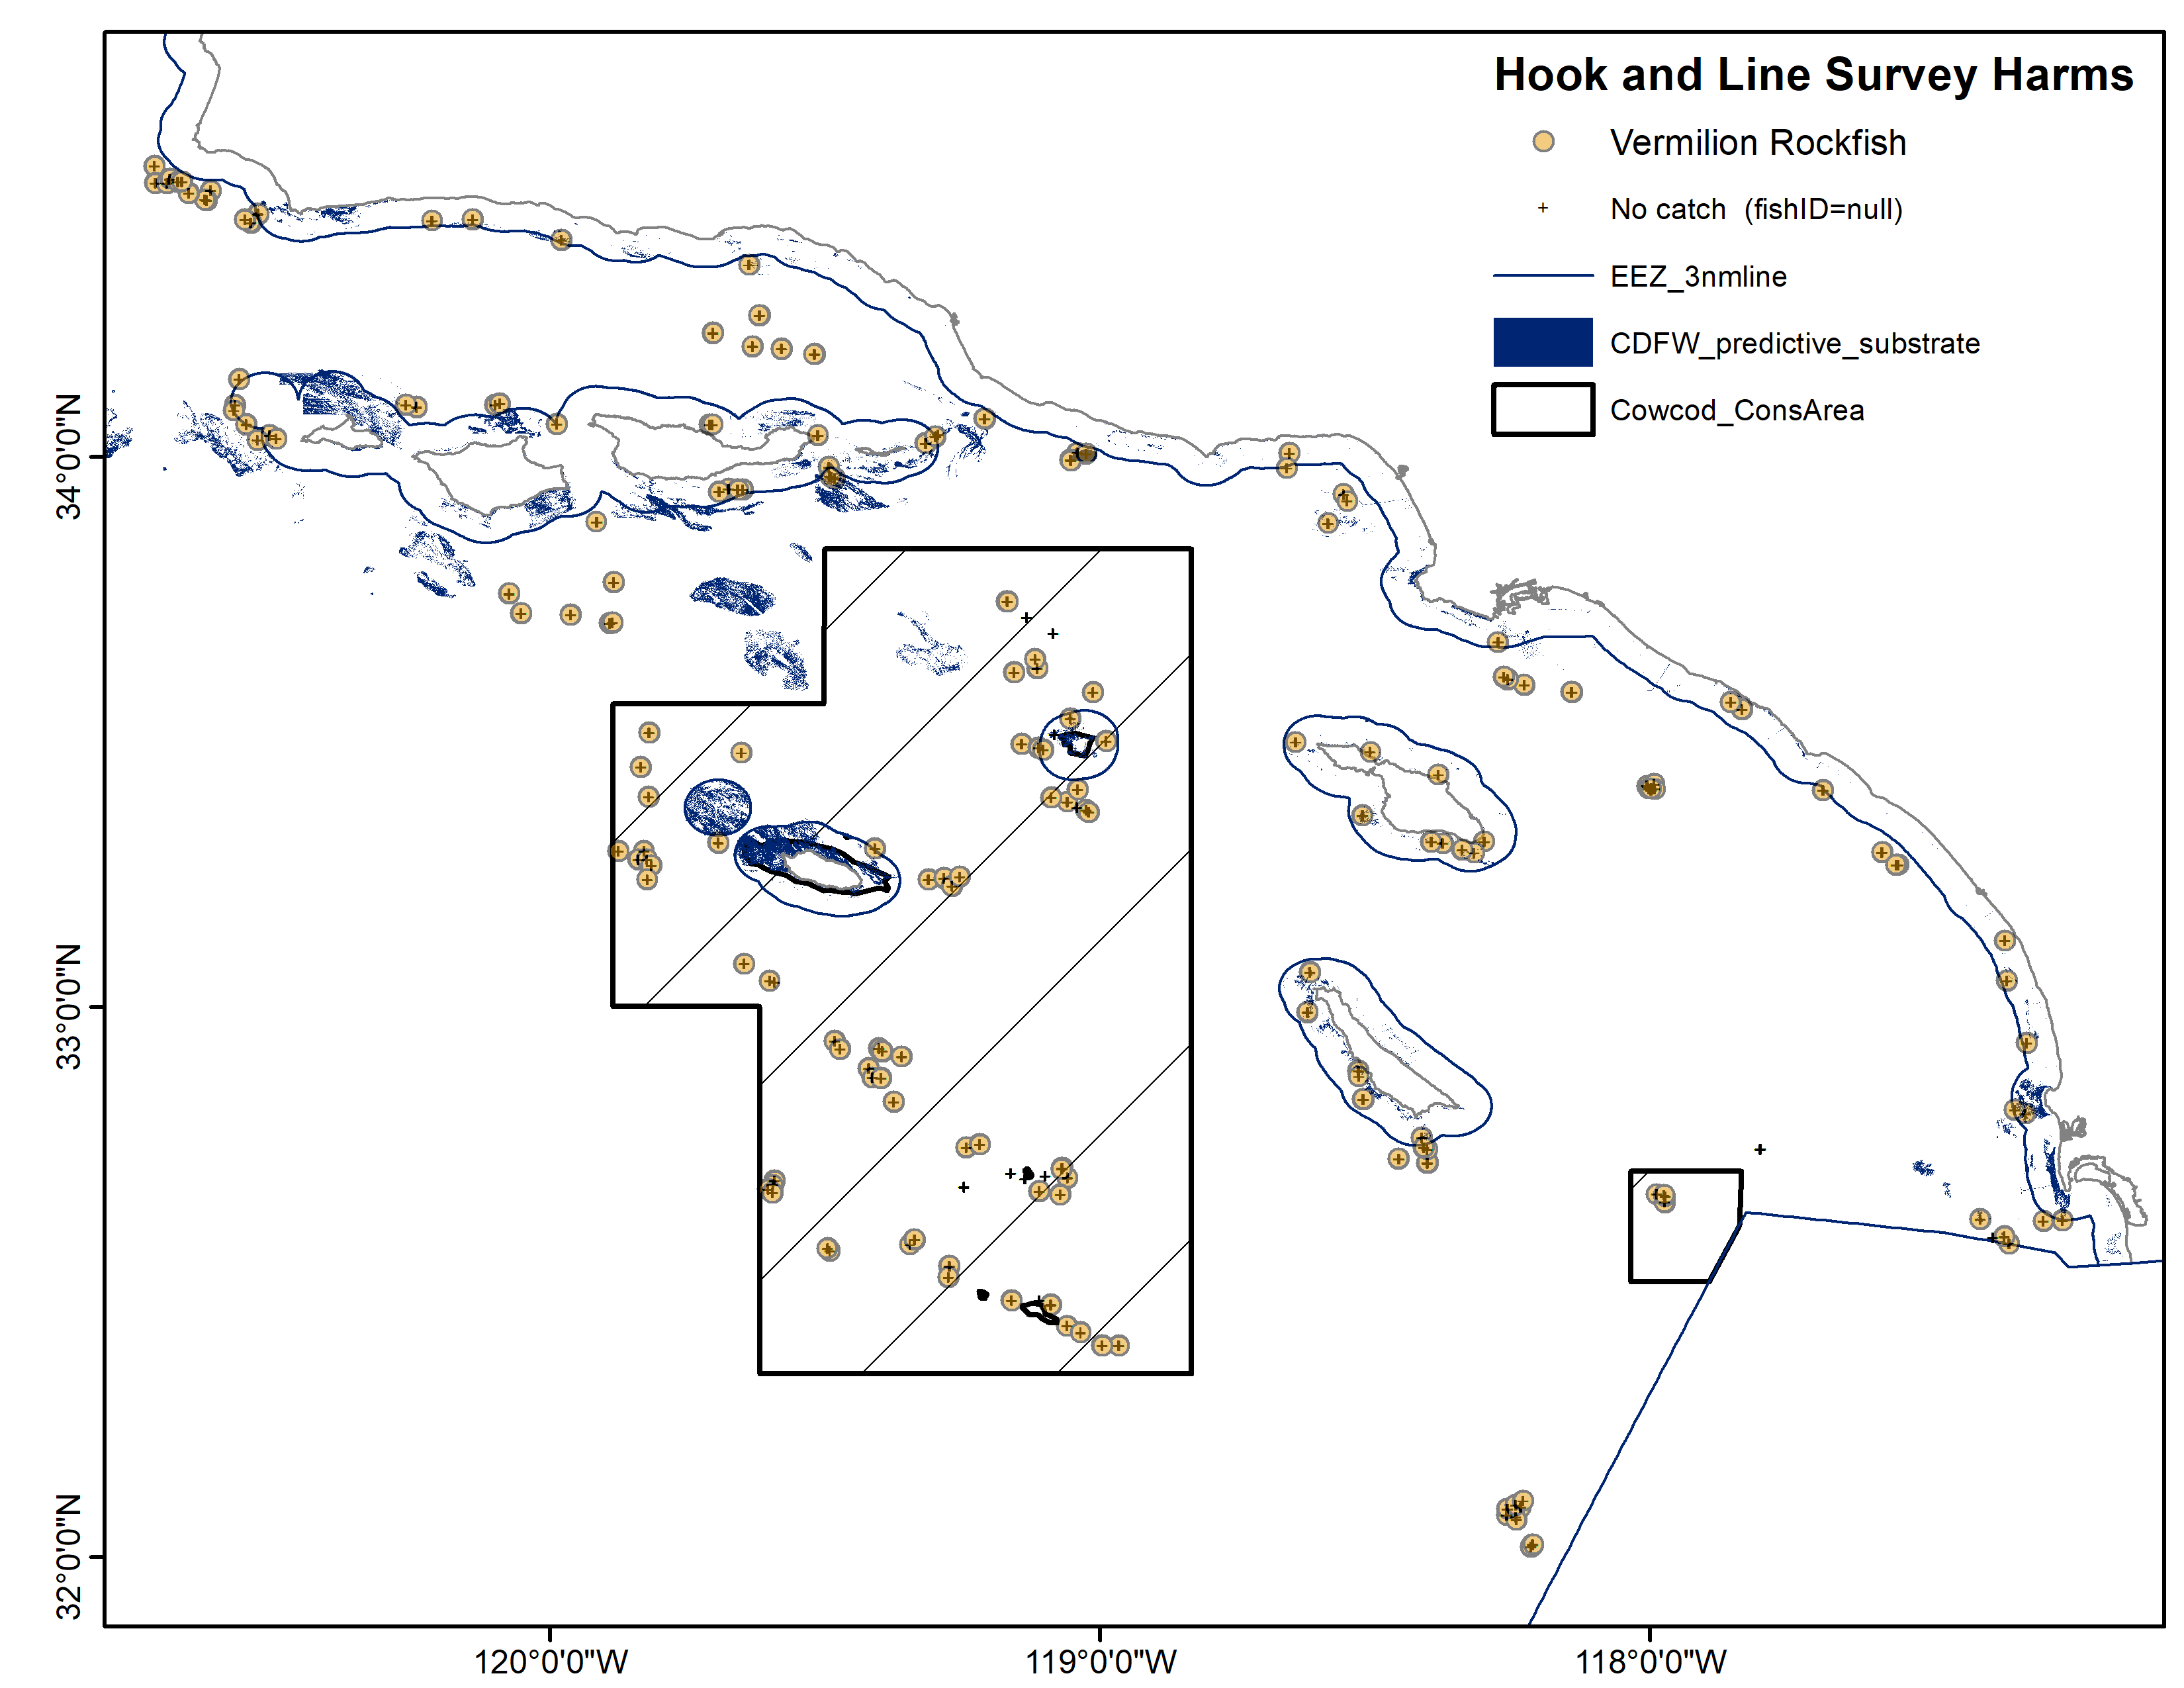
\includegraphics[width=0.85\linewidth]{C:/Stock_Assessments/VRML_Assessment_2021/Indices_of_Abundance/NWFSC_HL/HookandLine_Harms_CCA_Vermillion} \caption{Map of the NWFSC hook-and-line survey site with circle indicating location at which vermilion rockfish were observed at least once.}\label{fig:spp-sites}
\end{figure}

\FloatBarrier

\begin{figure}
\centering
\includegraphics{C:/Stock_Assessments/VRML_Assessment_2021/GitHub/Vermilion_2021/doc/indices/vermilion_NWFSC_HL_writeup_SCA_files/figure-latex/fig-posterior-mean-nwfschl-1.pdf}
\caption{\label{fig:fig-posterior-mean-nwfschl}Posterior predictive draws of the mean by year with a vertical line of the raw data average.}
\end{figure}

\FloatBarrier

\begin{figure}
\centering
\includegraphics{C:/Stock_Assessments/VRML_Assessment_2021/GitHub/Vermilion_2021/doc/indices/vermilion_NWFSC_HL_writeup_SCA_files/figure-latex/fig-posterior-sd-nwfschl-1.pdf}
\caption{\label{fig:fig-posterior-sd-nwfschl}Posterior predictive draws of the standard deviation by year with a vertical line representing the observed average.}
\end{figure}

\begin{figure}
\centering
\includegraphics{C:/Stock_Assessments/VRML_Assessment_2021/GitHub/Vermilion_2021/doc/indices/vermilion_NWFSC_HL_writeup_SCA_files/figure-latex/fig-propzero-nwfschl-1.pdf}
\caption{\label{fig:fig-propzero-nwfschl}Posterior predictive distribution of the proportion of zero observations in replicate data sets generated by the logit normal model with a vertical line representing the observed average.}
\end{figure}

\begin{figure}
\centering
\includegraphics{C:/Stock_Assessments/VRML_Assessment_2021/GitHub/Vermilion_2021/doc/indices/vermilion_NWFSC_HL_writeup_SCA_files/figure-latex/marginal2-nwfschl-1.pdf}
\caption{\label{fig:marginal2-nwfschl}Marginal effect of depth from a logit normal model without site.}
\end{figure}

\begin{figure}
\centering
\includegraphics{C:/Stock_Assessments/VRML_Assessment_2021/GitHub/Vermilion_2021/doc/indices/vermilion_NWFSC_HL_writeup_SCA_files/figure-latex/marginal-nwfschl-1.pdf}
\caption{\label{fig:marginal-nwfschl}Marginal effects from the final model logit normal model.}
\end{figure}

\begin{figure}
\centering
\includegraphics{C:/Stock_Assessments/VRML_Assessment_2021/GitHub/Vermilion_2021/doc/indices/vermilion_NWFSC_HL_writeup_SCA_files/figure-latex/fig-cpue-nwfschl-1.pdf}
\caption{\label{fig:fig-cpue-nwfschl}Standardized index and arithmetic mean of the CPUE from the filtered data. Each timeseries is scaled to its respective means.}
\end{figure}

\end{document}
